\chapter{DTLS} \label{Chp: DTLS}

In this chapter we analyse DTLS on Contiki. We consider only two ciphersuites those have been implemented by the tinydtls implementation, which are TLS\_PSK\_WITH\_AES\_128\_CCM\_8 and TLS\_ECDHE\_ECDSA\_WITH\_AES\_128\_CCM\_8. 

One thing to be noticed is that both ciphersuites uses AES-128 CCM for data encryption and therefore they only behave different during handshake. Hence we do not distinguish application data encrypted by both ciphersuites.

\section{DTLS Handshake}

\section{Packet Size}

Since application data are encrypted using AES-128 CCM, its size is not hidden and is visible in the header, as highlighted in the middle of \Cref{Fig: Size of application data in DTLS}.

\begin{figure*}[ht!]
	\center
	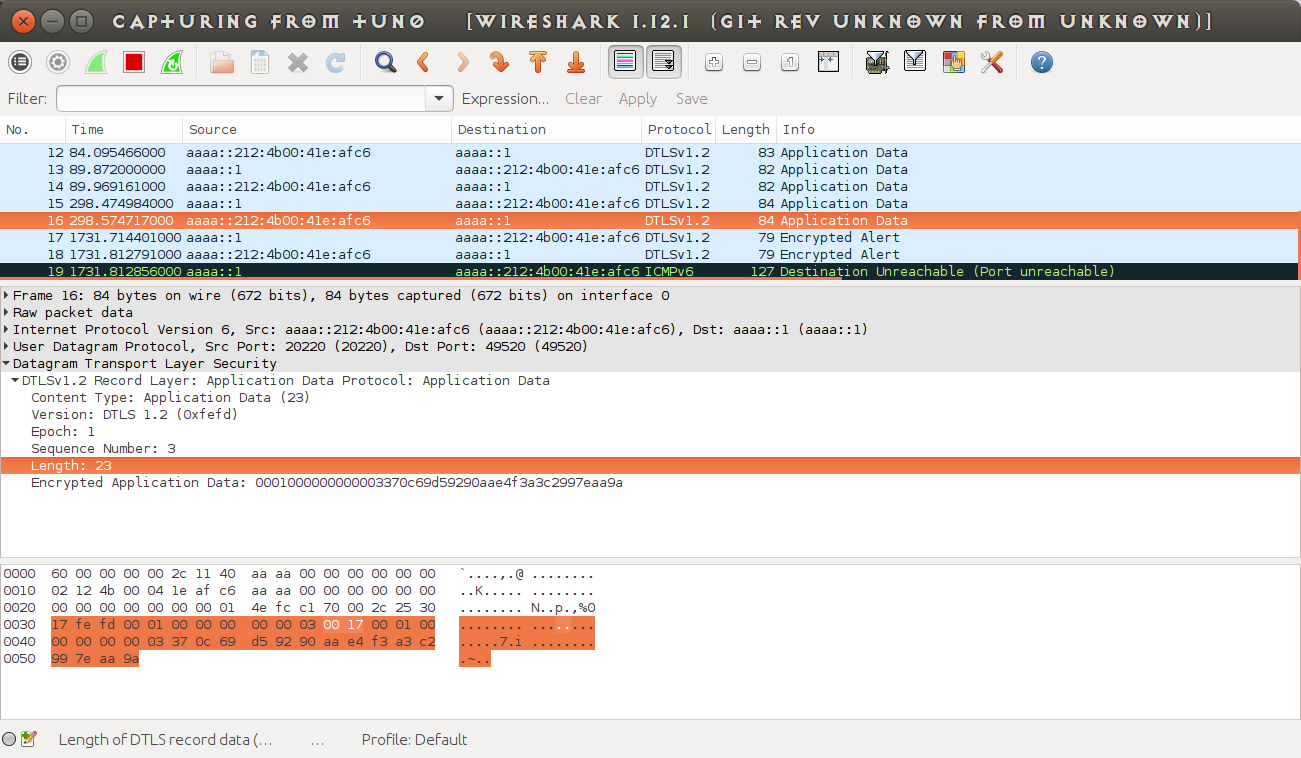
\includegraphics[width=.7\textwidth]{fig/dtlslength.png}
	\caption{Size of application data in DTLS}
	\label{Fig: Size of application data in DTLS}
\end{figure*}

Referring to \cite{rfc5116}, the size of application data is exactly the value of the highlighted Length in \Cref{Fig: Size of application data in DTLS} minus $16$ bytes.

%CoAP

\section{Timing}

In this section, we analyse the availability of timing information when the application data is protected by DTLS using the tinydtls implementation on Contiki.

\subsection{Processing Model}

The procedure of a Session with DTLS is as depicted by \Cref{Fig: A Session with DTLS}.

\begin{figure*}[ht!]
	\center
	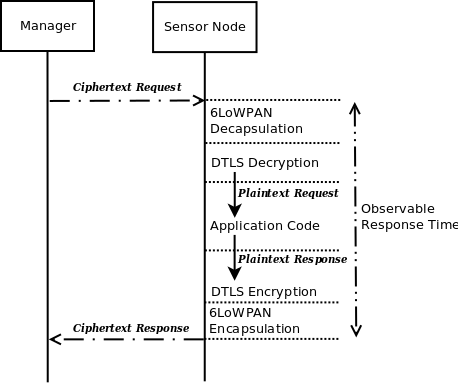
\includegraphics[width=0.8\textwidth]{fig/dtls_session.png}
	\caption{A Session with DTLS}
	\label{Fig: A Session with DTLS}
\end{figure*}

DTLS provides protection between only two Sensor Nodes in the network; thus the source and destination are consistent within a DTLS session. The 6LoWPAN encapsulation and decapsulation procedure are hence identical for all packets using the same DTLS session; therefore the time length of 6LoWPAN decapsulation and encapsulation in \Cref{Fig: A Session with DTLS} are considered to be constant.

Therefore in this section we put our interest in the timing of DTLS decryption/encryption and the execution time of application code.

\subsection{DTLS Encryption and Decryption}

\subsubsection{AES Timing}

tinydtls uses the OpenBSD optimised AES implementation. Its source code is available at:\\ 
\url{https://github.com/Salties/MyRepository/blob/master/tinydtls-0.8.2/aes/rijndael.c}

Inspecting the source code, we realised that there is no branch for AES-128 encryption as expected. This implies that its execution time is expected to be constant, regardless of the key and plaintext.

To verify this, we applied the similar TVLA-like test as described in \Cref{Sec: AES Timing}.

\subsubsection{Overall Timing}

\subsection{Application Code}




%DTLS has potentially the best interoperability as it is an variation of the widely used TLS in Internet. However, its design might not fit into the nature of WSN for practical reasons.
%
%\section{Implementation Issues}
%The most practical implementation we found on Contiki OS so far is tinydtls.
%
%tinydtls\cite{tinydtls} currently supports two ciphersuites, namely TLS\_PSK\_WITH\_AES\_128\_CCM\_8 and TLS\_ECDHE\_ECDSA\_WITH\_AES\_128\_CCM\_8. 
%
%However, we encountered several difficulties when trying to set up an encrypted network using tinydtls.
%
%\begin{description}
%\item[Low Computational Power] \hfill \\
%Curve computation requires relatively a large amount of computational power. Even using a relatively powerful platform (CC2538), it still takes minutes to complete a DTLS handshake with
%TLS\_ECDHE\_ECDSA\_WITH\_AES\_128\_CCM\_8.
%
%\item[Low Bandwidth] \hfill \\
%The 6LowPAN standard specifies that the minimum MTU is 127 bytes whilst 67 (87 with LLSEC) bytes are occupied by protocol headers until UDP, which leaves 60 (40 with LLSEC) bytes available for UDP layer payload. This value has been exceeded by several handshake packets even with pre-shared keys. Doing key exchange or even using longer keys only makes this problem worse. Some attempts have been made to solve this issue, e.g. CoDTLS\cite{CoDTLS}\footnote{This draft has been abandoned for some reason we do not know.}. As a result, DTLS is only available on those devices support extra frame length than 6LowPAN requirements.
%
%\item[Code Size] \hfill \\
%The tinydtls fails to fit into some devices, e.g. skymote, as its size of code is too large.
%\end{description}
%
%Therefore although TLS\_PSK\_WITH\_AES\_128\_CCM\_8 is less flexible (and probably less secure) as it uses a pre-shared master secret, it is still considered to be a relatively practical security measure as it requires less resources.
%
%\section{No Multicast Support}
%Some application protocols, such as CoAP, utilises the multicast feature of 6LowPAN whilst TLS is a protocol designated for securing communications between two parties, so is DTLS. To  our knowledge, DTLS does not make any attempt to support multicasting.
%
%\section{Overloading DTLS with LLSEC}
%Adopting both security measures at the same time is possible as they are implemented at different layers. However, it is questionable whether this will bring more security, as both {\it noncoresec} and TLS\_PSK\_WITH\_AES\_128\_CCM\_8 are using 128 bit AES with CCM mode as their cryptographic primitive.
